\documentclass{article}
\documentclass[a4paper,12pt]{article}
\usepackage[english]{babel}
\usepackage[utf8]{inputenc}
\usepackage{amsfonts}
\usepackage{indentfirst}
\usepackage[T1]{fontenc}
\usepackage{amsmath}
\usepackage{hyperref}
\usepackage{graphicx}
\usepackage{subfig}
\usepackage[export]{adjustbox}

\textwidth\paperwidth
\advance\textwidth -45mm
\oddsidemargin 18mm
\advance\oddsidemargin -18mm
\evensidemargin 18mm
\advance\evensidemargin -18mm
\topmargin -30mm
\advance\topmargin 17mm
\setlength\textheight{45\baselineskip}
\addtolength\textheight{\topskip}
\marginparwidth 15mm


\title{
\textbf{Human Recognition by Biometric Methods}\\
\bigskip
\textbf{Face detection and classification}\\
\bigskip
}
\author{Mikołaj Małkiński}
\date{7 June 2018}

\begin{document}

    \maketitle

    \section{Introduction}\label{sec:introduction}

    The goal of this task was to design, implement and train YOLO object detection system (YOLOv3 was chosen) for detecting faces of Polish rappers.
    Then, the extracted faces should be piped to previously trained model in order to classify them.

    The original dataset defined around 700 bounding boxes for faces.
    Several boxes could refer to the same image.
    The dataset was split automatically into two parts by Keras, using 80\% of the data for training and remaining 20\% for validation.

    The models are resizing the images before processing, so data of arbitrary size can be used.
    However, it is important to note that images have to be in the same format (\textit{jpg} used in this case).
    Therefore, part of the pre-processing involves converting images from \textit{png} format to \textit{jpg}.
    Lack of this conversion caused unbearable accuracy - close to 0\%.

    The project consists of following python scripts:
    \begin{itemize}
        \item \textit{yolo\_detect\_classify} - detects faces in image and predicts their classes,
        \item \textit{yolo\_evaluate} - evaluates model accuracy (Mean Average Precision at 0.5) and loss using specified configuration file,
        \item \textit{yolo\_reproduce\_results} - creates plots shown in the report,
        \item \textit{yolo\_train} - trains detection system using specified configuration file.
    \end{itemize}

    \section{Analysis of results}\label{sec:analysisOfResults}

    Figure~\ref{fig:configurations1} describes configurations used for analysis.
    Min and max input size define the range to vary the size of the image during training (should be a multiple of 32).
    Figure~\ref{fig:compare1} presents comparison of results using first and second configurations.
    It can be observed that although bigger input sizes resulted in faster mAP improvement, the final mAP@0.5 after 24 epochs rounded to 2 digits after the comma, was the same - $91\%$.
    However, Figure~\ref{fig:badResults} shows that the input size can't be too small.
    Unfortunately, the chosen model requires a substantial amount of graphics card memory (nearly 4GB were available), so larger batch sizes couldn't be tested.
    Finally, in the Figure~\ref{fig:bestConfig} the whole training process of the best performing configuration is presented.

    \begin{figure}[!h]
        \centering
        \begin{tabular}{cccc}
            \textbf{Configuration} & \textbf{Min input size} & \textbf{Max input size} & \textbf{Batch size} \\
            1 & 128 & 288 & 4 \\
            2 & 288 & 448 & 2 \\
            3 & 32 & 96 & 4 \\
        \end{tabular}
        \caption{Details of configurations}
        \label{fig:configurations1}
    \end{figure}

    \begin{figure}[!h]
        \centering
        \begin{tabular}{cc}
            \subfloat[Loss]{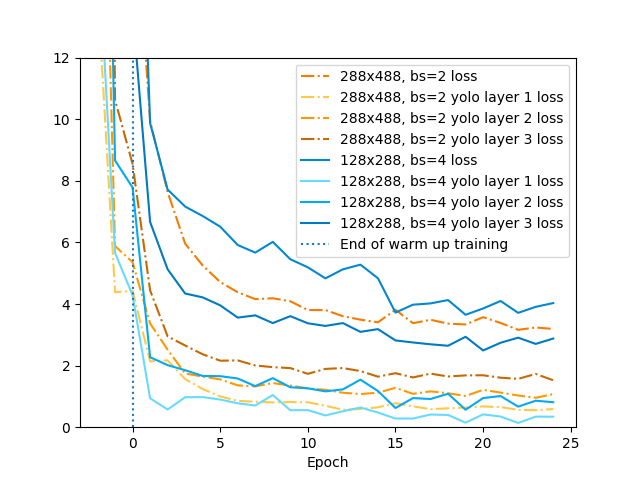
\includegraphics[width = 0.5\textwidth]{plots/compare_loss_face_01_06_15-25-face_05_06_15-08.png}} &
            \subfloat[Mean Average Precision at 0.5]{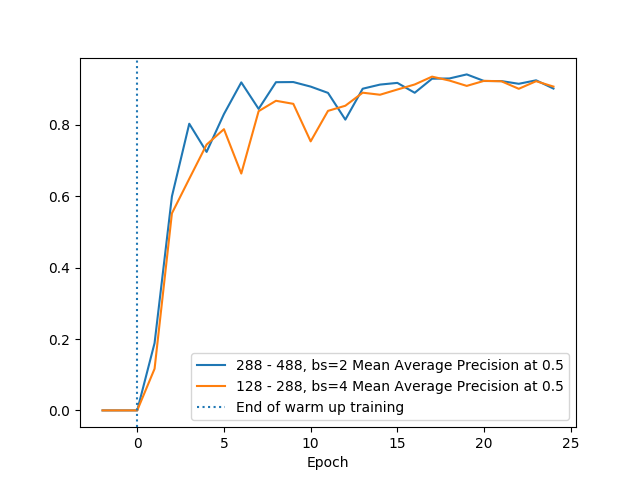
\includegraphics[width = 0.5\textwidth]{plots/compare_map_face_01_06_15-25-face_05_06_15-08.png}} \\
        \end{tabular}
        \caption{Comparison of two configurations}
        \label{fig:compare1}
    \end{figure}

    \begin{figure}[!h]
        \centering
        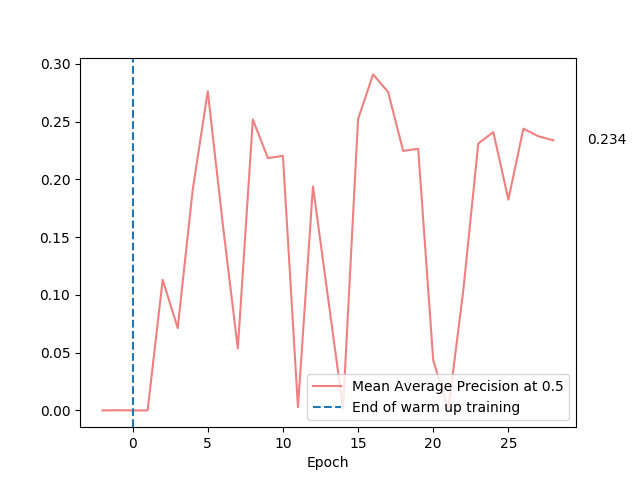
\includegraphics[width = 0.5\textwidth]{plots/yolo_hist_map_face_06_06_20-24.png}
        \caption{Mean Average Precision at 0.5 when input sizes are too small}
        \label{fig:badResults}
    \end{figure}

    \begin{figure}[!h]
        \centering
        \begin{tabular}{cc}
            \subfloat[Loss]{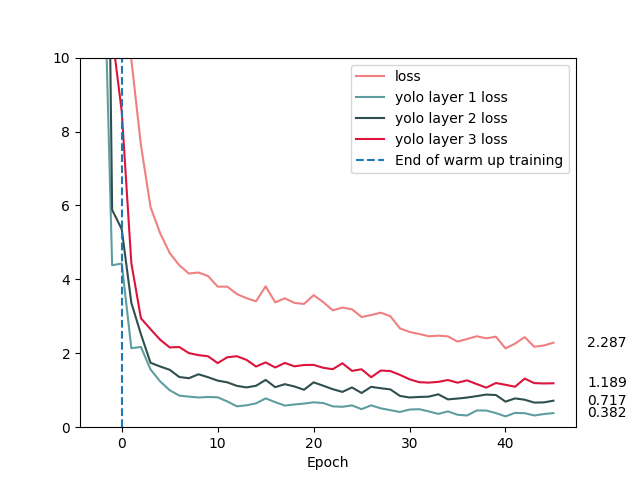
\includegraphics[width = 0.5\textwidth]{plots/yolo_hist_loss_face_01_06_15-25.png}} &
            \subfloat[Mean Average Precision at 0.5]{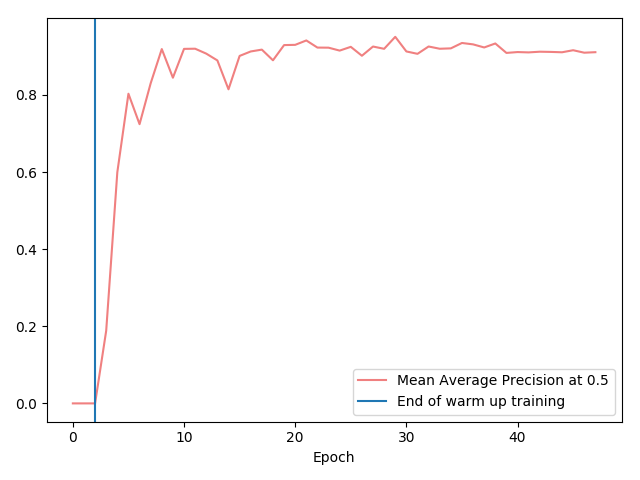
\includegraphics[width = 0.5\textwidth]{plots/yolo_hist_map_face_01_06_15-25.png}} \\
        \end{tabular}
        \caption{Results of the best performing configuration}
        \label{fig:bestConfig}
    \end{figure}

    \newpage

    \section{Examples of detection and classification}\label{sec:examplesOfDetectionAndClassification}

    The results of trained models are certainly satisfactory - 91\% mAP@0.5 for detection and close to 97\% for classification.
    Figures~\ref{fig:examples1} and~\ref{fig:examples2} shows how the whole pipeline performs on test images.
    It is worth observing, that this model works well with images of different resolution as well as objects varying in size.
    Obviously, since the classificator was trained to recognize only 4 people, some of the faces have wrong labels, simply because they weren't present in the dataset.
    Example of executed command to process the images, is presented below:
    \begin{verbatim}
python yolo_detect_classify.py -c yolo/configs/config_faces_01_06_15-25.json
-i ~/datasets/raw_dataset/ostr/505.jpg
    \end{verbatim}

    \begin{figure}[!h]
        \centering
        \begin{tabular}{cc}
            \subfloat[Blurry face]{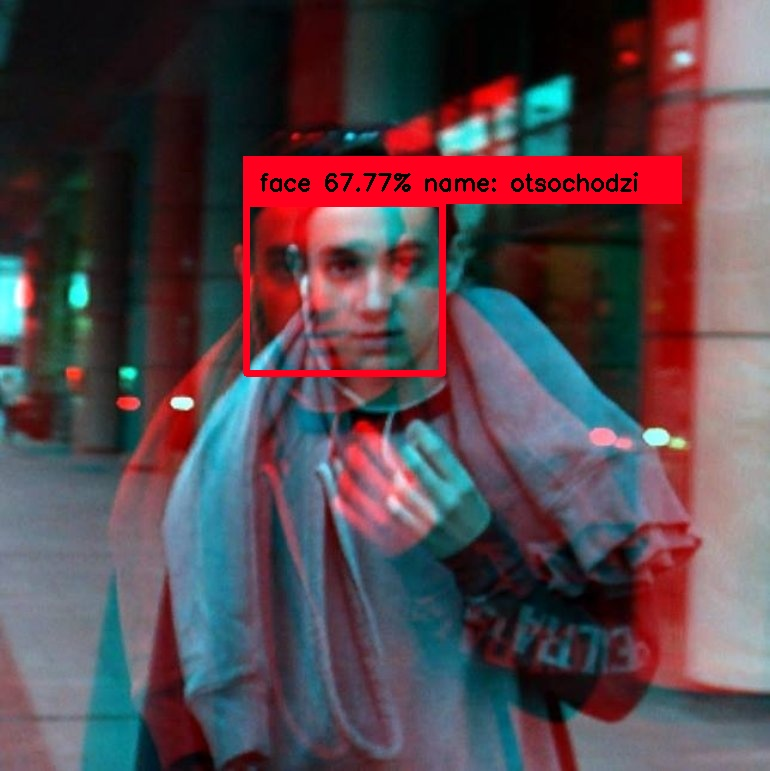
\includegraphics[width = 0.5\textwidth]{images/8.jpg}} &
            \subfloat[Partly hidden face]{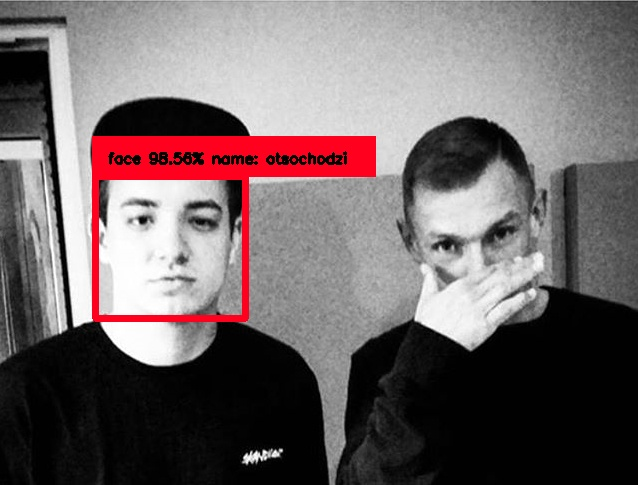
\includegraphics[width = 0.5\textwidth]{images/12.jpg}}} \\
            \subfloat[Woman face with longer hair]{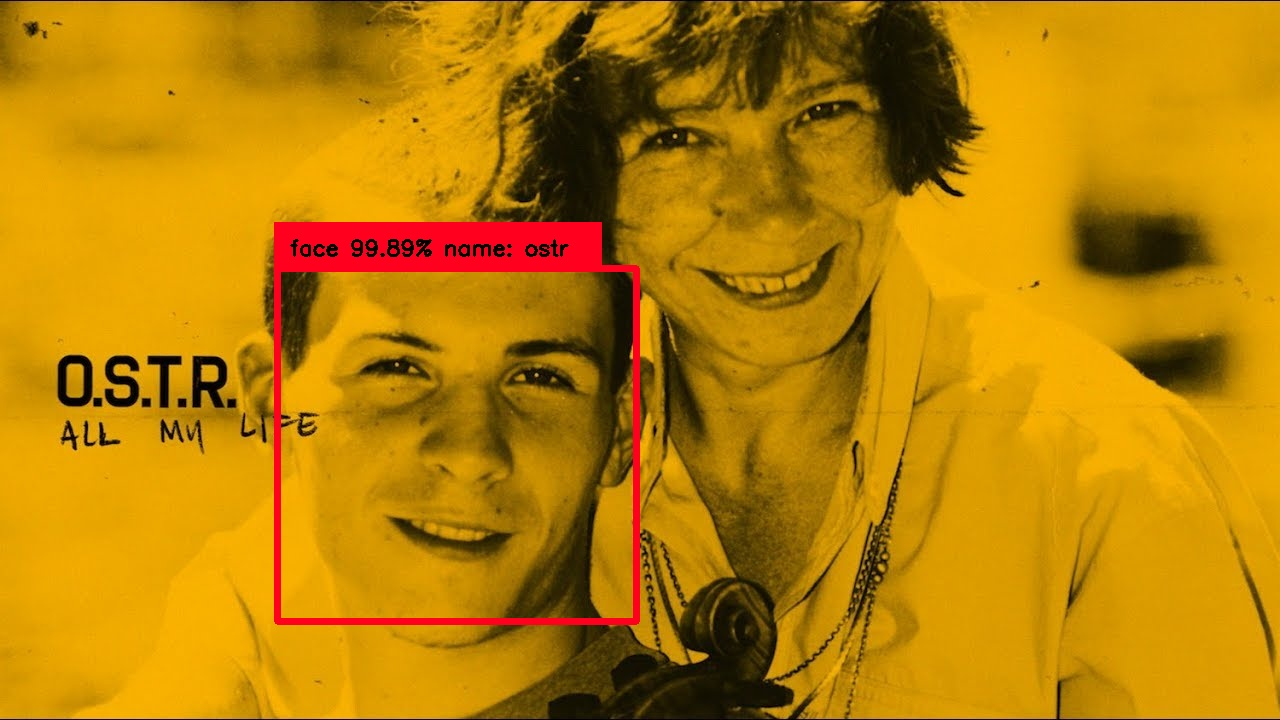
\includegraphics[width = 0.5\textwidth]{images/22.jpg}} &
            \subfloat[Small faces]{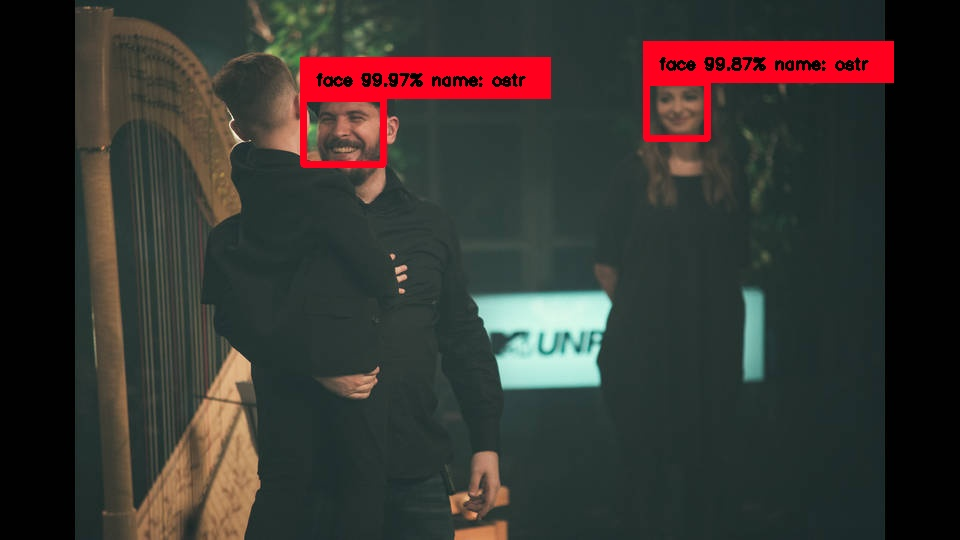
\includegraphics[width = 0.5\textwidth]{images/52.jpg}}} \\
            \subfloat[Faces of different size]{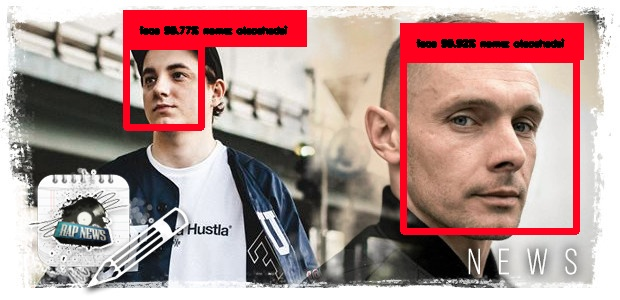
\includegraphics[width = 0.5\textwidth]{images/403.jpg}} &
            \subfloat[Similar faces]{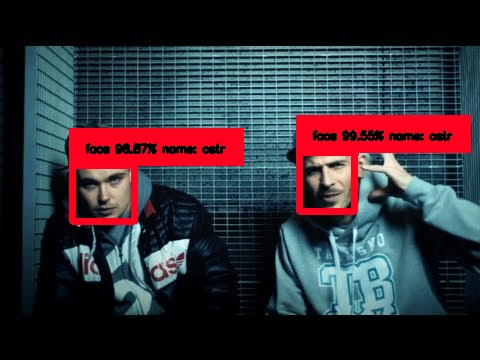
\includegraphics[width = 0.5\textwidth]{images/544.jpg}}} \\
        \end{tabular}
        \caption{Examples of detection and classification}
        \label{fig:examples1}
    \end{figure}
    \begin{figure}[!h]
        \centering
        \begin{tabular}{cc}
            \subfloat[Partly covered faces]{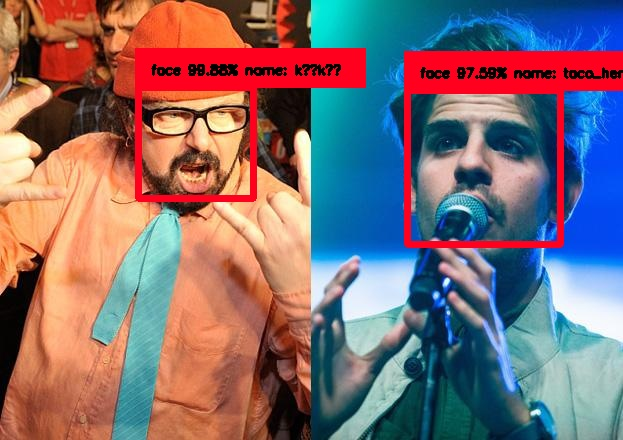
\includegraphics[width = 0.5\textwidth]{images/160.jpg}} &
            \subfloat[Clearly visible face]{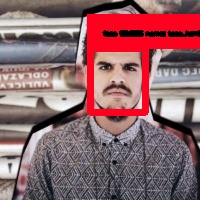
\includegraphics[width = 0.5\textwidth]{images/196.jpg}}} \\
            \subfloat[Face with glasses]{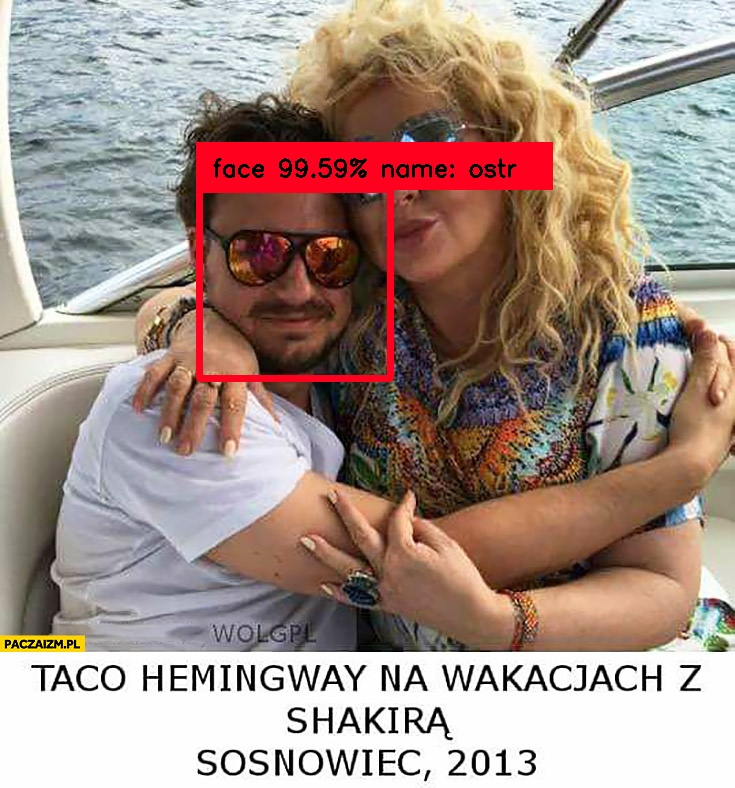
\includegraphics[width = 0.5\textwidth]{images/64.jpg}} &
            \subfloat[Normal faces]{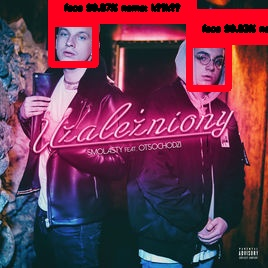
\includegraphics[width = 0.5\textwidth]{images/148.jpg}}} \\
        \end{tabular}
        \caption{Examples of detection and classification}
        \label{fig:examples2}
    \end{figure}

\end{document}
